\chapter{Evaluation}
\label{chapter|evaluation}

\section{Comparison of oro-server with other existing systems}
\label{sect|evaluation-oroserver}

\subsection{Performances Analysis}

\section{Experimental evaluation}
\label{sect|experimental-evaluation}

\subsection{Simulation of HRI interaction}
\label{sect|simulation}



\subsection{First Interaction Experiment}
\label{sect|expe1}

In order to illustrate the approach presented in this paper, we have designed
the following daily life situation. Tom and Jerry are moving to London, so they
are packing things in boxes. The scenario takes places in the living-room,
where Jido (our robot) is observing while they move things here and there. To
assess the reasoning abilities of the robot they ask Jido for information
(entered through keyboard). Ideally, the robot should also perform actions when
required (e.g. hand an object when asking ``give me...''). However, since it is
out of the scope of this work, we do not include any motion from the robot's
side.

Perception of objects is done through a tag-based system and humans are
detected through motion capture. The robot knowledge base is pre-loaded with
the \emph{ORO Commonsense Ontology}\footnote{This ontology can be downloaded
from \url{http://oro.openrobots.org/}.}.  We next describe in detail two
situations where we can follow the internal robot's reasoning and the
interaction with the users.

\subsubsection{Implicit disambiguation through visual perspective taking}

Tom enters the room while carrying a big box (Figure~\ref{fig|vpt}, page 1). He
approaches the table and asks Jido to handle him the video tape: ``Jido, can
you give me the video tape''. The \textsc{Dialogs} module queries the ontology to
identify the object the human is referring to: \stmt{?obj \textbf{type} VideoTape}. 

There are two video tapes in the scene: one on the table, and another one
inside the cardboard box. Thus, the knowledge base returns both: $\Rightarrow$
\stmt{?obj = [videoTape1, videoTape2]}. 

However, only one is visible for Tom (the one on the
table). Thus, although there is an ambiguity from the robot's perspective
(since it can see both video tapes), based on the perspective of its human
partner it infers that Tom is referring to the video tape on the table, and not
the one inside the box which is not visible from his view. Therefore,
non-visible objects are removed obtaining: \stmt{?obj =[videoTape1]}.

Since only one object is available, the robot infers
that the human refers to it and would eventually execute the command, \ie give
it to the human. Alternatively, the robot could first verify with the human if
that was the object being referred to or not before proceeding to execute the
action. Table~\ref{table|ptbeliefs} lists the robot's beliefs about itself and
its human partner involved in this situation.

\begin{table}
\begin{center}
\begin{tabular}{l}
\hline
Robot's beliefs about itself (\emph{robot's model}):\\
\hline
  \hspace{0.7cm}\stmt{videoTape1 \textbf{type} VideoTape}\\
  \hspace{0.7cm}\stmt{videoTape1 \textbf{isOn} table}\\
  \hspace{0.7cm}\stmt{videoTape1 \textbf{isVisible} \textit{true}}\\
  \hspace{0.7cm}\stmt{videoTape2 \textbf{type} VideoTape}\\
  \hspace{0.7cm}\stmt{videoTape2 \textbf{isIn} cardBoardBox}\\
  \hspace{0.7cm}\stmt{videoTape2 \textbf{isVisible} \textit{true}}\\
\hline
\hline
Robot's beliefs about Tom (\emph{Tom's model}):\\
\hline
  \hspace{0.7cm}\stmt{videoTape1 \textbf{type} VideoTape}\\
  \hspace{0.7cm}\stmt{videoTape1 \textbf{isOn} table}\\
  \hspace{0.7cm}\stmt{videoTape1 \textbf{isVisible} \textit{true}}\\
  \hspace{0.7cm}\stmt{videoTape2 \textbf{type} VideoTape}\\
  \hspace{0.7cm}\stmt{videoTape2 \textbf{isIn} cardBoardBox}\\
  \hspace{0.7cm}\stmt{videoTape2 \textbf{isVisible} \textit{false}}\\
 \hline
\end{tabular}
\end{center}
\caption{Robot's beliefs about itself and its human partner.}
\label{table|ptbeliefs}
\end{table}

\subsubsection{Explicit disambiguation through verbal interaction and gestures}
\begin{figure}[!ht]
  \centering
  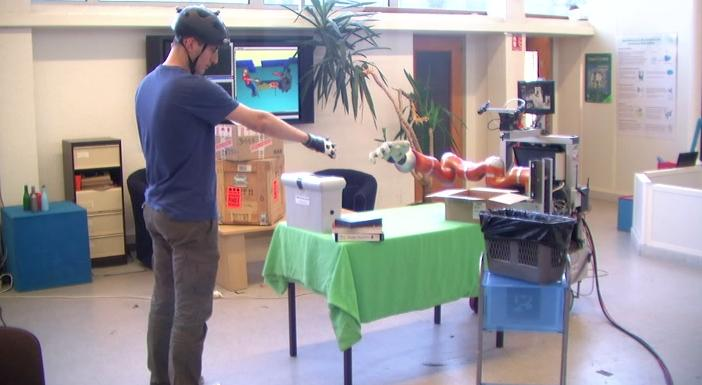
\includegraphics[width=0.9\linewidth]{images/dialogs/inTheBox2.jpg}
\caption{Jerry asks Jido for the content of the box by pointing at it.}
  \label{fig|pointing}
\end{figure}

In this situation, Jerry enters the
living room without knowing where Tom had placed the video tapes. So he first
asks Jido: ``What's in the box?''. Before the robot can answer the question it
has to figure out which box Jerry is talking about. Similar to the previous
situation, there are two available boxes: 

\begin{center}
\begin{tabular}{l}
\stmt{?obj \textbf{type} box}\\
\hspace{0.7cm}$\Rightarrow$ \stmt{?obj = [cardBoardBox, toolbox]}
\end{tabular}
\end{center}

However both are visible and the cognitive ambiguity resolution cannot be
applied. The only option is to ask Jerry which box he is referring to: ``Which
box, the toolbox or the cardboard box?'' Jerry could now simply answer the
question. Instead, he decides to point at it while indicating: ``This box''
(Figure~\ref{fig|pointing}). The robot's perception identifies the {\tt
cardBoardBox} as being pointed at and looked at by the human and updates the
ontology with this new information using a rule available in the commonsense
ontology ({\tt \textbf{pointsAt}(?ag, ?obj) $\land$ \textbf{looksAt}(?ag, ?obj) $\to$
\textbf{focusesOn}(?ag, ?obj)}) The \textsc{Dialogs} module is then able to merge both
sources of information, verbal (``this'') and gestural to distinguish the box
Jerry refers to.

\begin{center}
\begin{tabular}{l}
\stmt{Jerry \textbf{pointsAt} carboardBox}\\
\stmt{Jerry \textbf{looksAt} carboardBox}\\
$\to$ \stmt{Jerry \textbf{focusesAt} carboardBox}\\
\hspace{0.7cm}$\Rightarrow$ \stmt{?obj = [cardBoardBox]}
\end{tabular}
\end{center}

Finally, the \textsc{Dialogs} queries the ontology about the content of the box
and the question can be answered: ``Jido-E''. Note that the object's label is
used instead of its ID. This way we enhance interaction using familiar names
given by the users.

\begin{center}
\begin{tabular}{l}
\stmt{?obj \textbf{isIn} cardBoardBox}\\
\hspace{0.7cm}$\Rightarrow$ \stmt{?obj = videoTape2}\\
\end{tabular}
\end{center}

At this point Jerry wants to know where the other tape is, and that is exactly
what he asks Jido: ``And where is the other tape?''. In this occasion, the
\textsc{Dialogs} module is able to interpret that Jerry is not referring to the
video which they were just talking about, but to the other one:

\begin{center}
\begin{tabular}{l}
\stmt{?obj \textbf{type} VideoTape}\\
\stmt{?obj \textbf{differentFrom} videoTape2}\\
\hspace{0.7cm}$\Rightarrow$ \stmt{?obj = [videoTape1]}
\end{tabular}
\end{center}

Since there is only one possible ``other'' video (there are only two videos in
the scene), it can directly answer Jerry: ``The other tape is on the table and
next to the toolbox.''

\begin{center}
\begin{tabular}{l}
\stmt{videoTape1 \textbf{isOn} table}\\
\stmt{videoTape1 \textbf{isNextTo} toolbox}
\end{tabular}
\end{center}




\subsection{User studies}
\label{sect|userstudies}


